\documentclass[journal]{IEEEtran}

\usepackage[T1]{fontenc}
\usepackage[utf8]{inputenc}
\usepackage[spanish,es-noquoting,es-nolists,es-noshorthands]{babel}
\usepackage{amsmath,amssymb}
\usepackage{booktabs}
\usepackage{cite}
\usepackage{url}
\usepackage{graphicx}
\usepackage[hidelinks]{hyperref}
\graphicspath{{figuras/}}
\renewcommand{\IEEEkeywordsname}{Palabras clave}
\addto\captionsspanish{\renewcommand{\tablename}{Tabla}}

\begin{document}

\title{Estructura frente a tamaño: selección de conjuntos críticos
en el grafo de exposición de DeFi}

\author{David Sánchez Lombana \quad Juan Sebastián Cuesta Montenegro\\[2pt]
{\small\texttt{davidh.sanchez@urosario.edu.co} \quad
\texttt{juans.cuesta@urosario.edu.co}}\\[2pt]
{\small Universidad del Rosario, Bogotá, Colombia}%
\thanks{Proyecto final del curso de Teoría de Grafos, 2026-II.
Profesor: Daniel Bojacá. Entrega final.}}

\pagestyle{plain}

\maketitle

\begin{abstract}
Los protocolos de finanzas descentralizadas (DeFi) se prestan y se respaldan
unos a otros, así que la caída de uno puede arrastrar a otros. Hoy, para
estudiar ese riesgo se escogen los protocolos más grandes. Este trabajo pregunta
si hay una mejor forma de escogerlos: mirar cómo están conectados. Comparamos
cuatro criterios estructurales (intermediación, articulación, conjunto dominante
conectado e inmunización espectral) contra dos de tamaño (fuerza de exposición y
PageRank) sobre datos reales de 2022 a 2024. Los criterios estructurales parten
más la red, pero lo que separan son protocolos pequeños; los de tamaño quitan
más exposición. Las dos visiones responden preguntas distintas. Publicamos la
herramienta que hace el análisis.
\end{abstract}

\begin{IEEEkeywords}
Teoría de grafos, fragmentación de redes, conjunto dominante conectado,
puntos de articulación, robustez de redes, finanzas descentralizadas.
\end{IEEEkeywords}

\section{Introducción}

\IEEEPARstart{L}{a} propiedad que distingue a las finanzas descentralizadas
(DeFi) de la banca tradicional es la \emph{composabilidad}: cualquier protocolo
puede integrar a otro sin permiso previo, de modo que el activo que un protocolo
emite se convierte en el colateral que otro acepta \cite{capponi2023defi}. Un
depósito puede ser representado por un token, ese token depositado en un segundo
protocolo como garantía de un préstamo, y el resultado reutilizado en un tercero.
El efecto agregado es una red de dependencias en la que el valor de un protocolo
depende del valor de activos emitidos por otros, y en la que un choque sobre un
solo activo puede propagarse en cascada por toda la red \cite{shu2026dexposurefm}.

Esta estructura es, de forma natural, un grafo: los protocolos son los vértices y
las relaciones de exposición son las aristas dirigidas y ponderadas. La literatura
de redes financieras estableció hace más de una década que la topología de esa red
--y no solo el tamaño de sus participantes-- determina si un choque se amortigua o
se amplifica. El resultado central de Acemoglu \emph{et al.}
\cite{acemoglu2015systemic} es una transición de fase: una red densamente conectada
es más resiliente que una dispersa frente a choques pequeños, y más frágil frente a
choques grandes. Jackson y Pernoud \cite{jackson2020survey} organizan el campo, y
Bardoscia \emph{et al.} \cite{bardoscia2021physics} revisan el aparato de física de
redes que se le ha aplicado.

Hasta hace poco, aplicar ese aparato a DeFi era inviable porque el grafo no
existía: había que reconstruirlo desde los registros de las cadenas de bloques.
Eso cambió en noviembre de 2025, cuando Wu \emph{et al.} publicaron
\emph{DeXposure} \cite{wu2025dexposure}, el primer conjunto de datos a gran escala
de exposición crediticia entre protocolos, con 43{,}7 millones de registros que
cubren más de 4\,300 protocolos y 602 cadenas, junto con su código. Tres meses
después, el mismo grupo publicó un modelo fundacional de grafos temporales sobre
esos datos \cite{shu2026dexposurefm}.

Con el grafo disponible y su modelado predictivo ocupado, queda abierta una
pregunta que es estrictamente de teoría de grafos y que ninguno de los dos
trabajos aborda. Ambos caracterizan el grafo mediante métricas descriptivas
--grado, entropía, asortatividad, cercanía, agrupamiento-- y el segundo somete la
red a pruebas de estrés, pero en todos los casos \emph{los nodos que se golpean se
eligen por tamaño o categoría}: el protocolo con mayor valor bloqueado, los cinco mayores,
o un sector completo. Ningún escenario selecciona los nodos por su posición
estructural en el grafo. La pregunta que este proyecto plantea es la inversa:

\begin{quote}
\emph{Dado un presupuesto de $k$ protocolos, ¿qué criterio de selección
identifica al conjunto cuya caída simultánea fragmenta más el sistema, y
coincide ese conjunto con los protocolos más grandes?}
\end{quote}

Formulada así, la pregunta pertenece a un problema clásico: el de la
\emph{fragmentación de redes} por remoción dirigida de vértices. Como generador
de candidatos se propone el \emph{conjunto dominante conectado}. Un conjunto dominante conectado (CDS) de un grafo es un subconjunto
de vértices que induce un subgrafo conexo y tal que todo vértice fuera de él es
adyacente a alguno de sus miembros; funciona como una columna vertebral de
comunicación \cite{guha1998approximation}. Aquí se evalúa si esa columna vertebral
contiene buenos candidatos para un ataque. Es una hipótesis experimental: un CDS
no es necesariamente un corte de vértices y su garantía de aproximación no se
transfiere al daño causado al removerlo.

Existe un precedente metodológico directo en otro dominio. Koç \emph{et al.}
\cite{koc2014topological} estudian las transiciones de fase en fallas en cascada
en redes eléctricas comparando tres métricas espectrales --radio espectral,
resistencia efectiva de grafo y conectividad algebraica-- contra el umbral crítico
de carga, y atacan la red mediante remoción dirigida por intermediación. Su
hallazgo es pertinente: la conectividad algebraica \cite{fiedler1973algebraic}
captura el comportamiento de la cascada con una correlación cercana al 90\,\%,
mientras que el radio espectral alcanza aproximadamente el 50\,\% en ese diseño.
Este antecedente motiva comparar estrategias de remoción; aquí se mide
fragmentación estática, sin simular la dinámica física de una cascada eléctrica.

\section{Descripción del problema}

\subsection{Modelo}

Para cada instante $t$ se define el grafo dirigido y ponderado
\begin{equation}
G_t = (V_t, E_t, w_t),
\label{eq:modelo}
\end{equation}
donde $V_t$ es el conjunto de protocolos activos en $t$; una arista
$(u,v) \in E_t$ indica que el protocolo $u$ mantiene exposición crediticia frente
al protocolo $v$, es decir, que parte del valor que $u$ custodia depende de
activos emitidos o respaldados por $v$; y $w_t(u,v) \in \mathbb{R}_{>0}$ es la
magnitud de esa exposición. La relación no es simétrica: que $u$ dependa de $v$ no
implica lo recíproco, por lo que el grafo es genuinamente dirigido. Se denota por
$\tilde{G}_t$ su simetrización, empleada cuando la propiedad de interés es la
conectividad y no el sentido de la propagación.

\subsection{Caracterización empírica de la instancia}

La instancia es el panel semanal
publicado con \emph{DeXposure} \cite{wu2025dexposure}, cuyas dimensiones se
verificaron directamente sobre los datos y se resumen en la Tabla~\ref{tab:datos}.

\begin{table}[!t]
\renewcommand{\arraystretch}{1.25}
\caption{Dimensiones del panel de exposición inter-protocolo}
\label{tab:datos}
\centering
\setlength{\tabcolsep}{5pt}
\begin{tabular}{ll}
\toprule
\textbf{Propiedad} & \textbf{Valor} \\
\midrule
Instantáneas semanales      & 314 \\
Cobertura temporal          & 2018-04-23 a 2024-04-29 \\
Registros de arista         & 1\,258\,297 (52\,416 lazos) \\
Vértices distintos sin lazos & 3\,899 \\
Pares dirigidos distintos   & 37\,604 \\
Vértices por instantánea (2022--2024) & 1\,062 -- 3\,016 \\
Reciprocidad binaria (2022--2024) & 0{,}08 -- 0{,}19 \\
Componentes conexas (2022--2024)  & 3 -- 21 \\
Componente gigante (2022--2024)   & 98{,}0\,\% -- 99{,}8\,\% de los vértices \\
\bottomrule
\end{tabular}
\end{table}

Las cuatro últimas filas se reportan sobre el período 2022--2024, en el que el
grafo ya alcanzó su tamaño maduro; antes de 2022 la red tiene menos de mil
vértices y sus valores no son comparables.
Dos hechos de esa caracterización
condicionan el diseño. El primero es que el grafo \emph{no} es conexo: se
descompone en entre 3 y 21 componentes, de las cuales una concentra entre el
98\,\% y el 99{,}8\,\% de los vértices y el resto son fragmentos diminutos. Por eso el segundo valor propio de
la matriz laplaciana del grafo completo (su conectividad algebraica) es 0 y no
aporta información; el análisis debe restringirse a la componente gigante, y el número de
componentes pasa a ser una variable de interés por derecho propio. El segundo es
que la reciprocidad es baja pero no despreciable, lo que obliga a justificar
explícitamente cada paso en que se simetrice el grafo.

\subsection{Formulación}

Sea $\tilde G_t=(V_t,\tilde E_t)$ la proyección no dirigida de una instantánea,
definida en \eqref{eq:proyeccion}, y sea $C_t$ su componente mayor por número de
vértices. El experimento se realiza sobre $H_t=\tilde G_t[C_t]$; los fragmentos
preexistentes se describen por separado. Para $S\subseteq C_t$, $H_t-S$ elimina
los vértices de $S$ y sus aristas incidentes. La proyección $\tilde G_t$ se usa
solo para determinar la conectividad. Los pesos y las direcciones se toman
siempre del grafo dirigido original $G_t[C_t]$, cuyas aristas $E_t$ conservan
cada sentido de exposición por separado.

\paragraph{Observación diagnóstica} Preguntar por el menor conjunto de vértices
que \emph{desconecta} la red no tiene interés en esta instancia. En las 13
semanas analizadas, entre el 37 y el 45\,\% de los vértices de la componente
gigante son hojas (vértices de grado 1), y retirar el único vecino de una hoja
ya la aísla. Por tanto, $\kappa(H_t)=1$: basta un vértice para desconectar
$H_t$, aunque ese corte solo separe a un protocolo marginal. Desconectar no
equivale a fragmentar. La pregunta pertinente es cuánto daño causa un
presupuesto dado.

\paragraph{Fragmentación con presupuesto} El problema que este trabajo aborda es,
dado un presupuesto de $k$ protocolos, hallar el conjunto que maximiza el daño:
\begin{equation}
S^{\ast}_{k,j}\in\arg\min_{S\subseteq C_t,\ |S|=k}D_j(H_t-S),
\quad j\in\{\mathrm{est},\mathrm{pond}\}.
\label{eq:optimo}
\end{equation}
Aquí $1\leq k<|C_t|$ y $D_j$ mide cuánto conserva la red tras la remoción
(una retención): minimizarla maximiza su pérdida. Se plantean dos objetivos separados, cuyos óptimos pueden diferir.
La variante estructural, que minimiza el número de vértices de la componente
mayor, es NP-dura \cite{shen2012interdiction}. Para la variante ponderada no se
demuestra aquí la NP-dureza: requeriría una reducción que no es inmediata,
porque con pesos unitarios $D_{\mathrm{pond}}$ cuenta las aristas internas de
la componente, no sus vértices, y minimizar una cantidad no equivale a
minimizar la otra. En cualquier caso, el tamaño de la instancia impide la
búsqueda exhaustiva: con $|C_t|\approx2\,000$ y $k=10$ hay del orden de
$10^{26}$ conjuntos candidatos. También es NP-dura la construcción del conjunto dominante
conectado de cardinalidad mínima, para el cual Guha y Khuller
\cite{guha1998approximation} proporcionan algoritmos de aproximación con garantía
logarítmica. La intratabilidad es lo que lo hace interesante como proyecto de
teoría de grafos: obliga a implementar y comparar aproximaciones y heurísticas en
lugar de resolver el óptimo.

\subsection{Dos medidas de daño, y por qué no basta una}

Sea $\mathcal K(H_t-S)$ la familia de componentes conexas restantes y, para
$U\subseteq C_t$, defínase la exposición interna dirigida
\begin{equation}
W_t(U)=\sum_{(u,v)\in E_t\cap(U\times U)}w_t(u,v),
\qquad W_0=W_t(C_t).
\label{eq:peso-interno}
\end{equation}
Cada arista dirigida se cuenta una vez; las aristas recíprocas son registros
distintos. Las dos cantidades retenidas son
\begin{equation}
\begin{aligned}
D_{\mathrm{est}}(H_t-S)&=\max_{Q\in\mathcal K(H_t-S)}|Q|,\\
D_{\mathrm{pond}}(H_t-S)&=\frac{\max_{Q\in\mathcal K(H_t-S)}W_t(Q)}{W_0}.
\end{aligned}
\label{eq:medidas}
\end{equation}
La primera cuenta vértices; la segunda mide la mayor exposición interna que
queda reunida en una sola componente. La componente que maximiza el peso puede
ser distinta de la que maximiza la cardinalidad.
Con pesos positivos, ambas cantidades de \eqref{eq:medidas} son no crecientes
al ampliar $S$: cada componente posterior está contenida en una anterior.
Si $W_0=0$, solo se evalúa el objetivo estructural.

Contar protocolos y sumar exposición responden a preguntas diferentes: una
componente con muchos vértices puede tener menos peso que una más pequeña.
Se reportan ambas medidas y se toma la ponderada como principal. Ésta mide
concentración de exposición conectada, no pérdidas monetarias realizadas ni
tamaño de una cascada; la estructural permite el contraste con la literatura
de robustez de redes \cite{albert2000error}. Los porcentajes de concentración
se calcularán indicando semana, población y denominador, sin equiparar una suma
de fuerzas de vértices con una suma de aristas.

\subsection{Criterios de selección en competencia}

El aporte del proyecto es comparar, sobre la misma instancia y el mismo
presupuesto $k$, criterios de selección procedentes de tradiciones distintas:

\begin{enumerate}
\item \textbf{Fuerza de exposición}: los $k$ vértices de mayor suma de pesos
      incidentes. Es un control de escala de exposición, distinto del TVL.
\item \textbf{Centralidad de intermediación} \cite{freeman1977betweenness}, la
      estrategia de ataque empleada por Koç \emph{et al.}
      \cite{koc2014topological}.
\item \textbf{PageRank}, por ser el componente estructural del índice de
      importancia sistémica de \cite{shu2026dexposurefm}.
\item \textbf{Puntos de articulación}, el criterio de conectividad puro.
\item \textbf{Conjunto dominante conectado}, construido con el algoritmo de
      aproximación de Guha y Khuller \cite{guha1998approximation}.
\item \textbf{Inmunización espectral}, adaptación voraz al grafo dirigido y
      ponderado del objetivo de reducir el radio espectral \cite{chen2016node}.
\end{enumerate}

Como controles adicionales se incluirán rankings por TVL y por una
implementación declarada del SIS de DeXposure-FM \cite{shu2026dexposurefm},
cuando se disponga de sus insumos contemporáneos. Comparar solo contra fuerza
o PageRank no permite afirmar que se supera al TVL ni al SIS completo.

\subsection{Motivación preliminar del contraste con tamaño}

Una medición preliminar propia sobre las 174 instantáneas posteriores a enero de
2021 motiva la pregunta. El cálculo exploratorio usó la componente gigante y
pesos transformados con $\log(1+w)$, y debe distinguirse de la evaluación
financiera con pesos crudos. Al regresar el logaritmo de cada invariante contra los
logaritmos del número de vértices y de aristas se obtiene que la resistencia
efectiva de grafo queda explicada por el tamaño con $R^2 = 1{,}000$ y el radio
espectral con $R^2 = 0{,}987$; la conectividad algebraica, en cambio, solo con
$R^2 = 0{,}455$. Estos ajustes describen asociación dentro de esa muestra;
un $R^2$ alto, o redondeado a uno, no demuestra una identidad matemática ni
ausencia de información adicional. Son resultados preliminares que deberán
acompañarse de código, especificación de matrices y salida verificable antes
de usarse como evidencia definitiva. Motivan comparar directamente los conjuntos
de remoción, sin anticipar qué ranking será superior.

\subsection{Alcance y limitaciones asumidas}

El proyecto se acota deliberadamente. No se propone construir el grafo, que ya
existe \cite{wu2025dexposure}, ni predecir su evolución, que ya se hace
\cite{shu2026dexposurefm}. El peso de arista de
$D_{\text{pond}}$ es el de exposición del propio panel, no el valor total
bloqueado, porque Luo \emph{et al.} \cite{luo2024piercing} demostraron que esa
métrica está inflada por doble conteo. Se asumen tres limitaciones desde el
planteamiento: la resolución temporal es semanal, mientras que las cascadas de
liquidación ocurren en minutos; se preseleccionan tres episodios históricos,
insuficientes para inferir poder predictivo general; y el grafo es endógeno al riesgo, pues los protocolos
eligen a quién exponerse y un protocolo puede ser central precisamente porque se
le considera seguro.

\subsection{Validación externa disponible}
\label{sec:validacion}

Que tres episodios no permitan un diseño estadístico no significa que no
permitan nada: admiten un \emph{estudio de caso}, y son la única validación
externa prevista para este proyecto. La pregunta es si el conjunto heurístico
$S_{a,k}$ producido por cada método $a$ sobre la instantánea inmediatamente anterior a cada
episodio --Terra/Luna en mayo de 2022, FTX en noviembre de 2022 y la pérdida de
paridad de USDC en marzo de 2023-- contiene a los protocolos que efectivamente
resultaron afectados.

Dos precisiones metodológicas, ambas obligadas por lo que muestran los datos. La
primera es que la verdad de campo \textbf{no} puede ser la desaparición del
protocolo del grafo: un protocolo puede seguir registrado después de sufrir
una pérdida. Se usarán informes públicos para identificar afectados y la caída
de fuerza de exposición como indicador complementario, sin equiparar cualquier
caída de exposición con insolvencia. La ventana y el umbral se fijarán antes
del cotejo. La
segunda es que la lista de protocolos afectados se curará a mano a partir de
informes públicos posteriores a cada episodio, y no por coincidencia de cadenas
de texto en el nombre: una búsqueda por patrón sobre los nombres devuelve falsos
positivos evidentes como \emph{Nexus Mutual}, \emph{NFTX} o \emph{Solana
Farm}. Esa lista no se alcanzó a armar; la Sección~\ref{sec:caso} usa solo
la caída de exposición.

\section{Objetivos}

\subsection{Objetivo general}

Determinar, mediante algoritmos de teoría de grafos y para un presupuesto dado
de protocolos, los conjuntos cuya remoción fragmenta en mayor medida el grafo de
exposición inter-protocolo de las finanzas descentralizadas, y evaluar si los
criterios estructurales de selección superan a los criterios basados en tamaño
que emplea actualmente el estado del arte.

\subsection{Objetivos específicos}

\begin{enumerate}
\item \textbf{Modelar} el panel semanal de exposición inter-protocolo como una
      familia de grafos dirigidos y ponderados, estableciendo de forma explícita
      el criterio de arista, la métrica de peso y el tratamiento de la
      componente gigante y de los fragmentos.

\item \textbf{Caracterizar} cada instantánea mediante invariantes de conectividad
      --número de componentes, tamaño de la componente gigante, conectividad
      algebraica, distribución de grados y concentración del peso de exposición--
      y documentar su evolución entre 2018 y 2024.

\item \textbf{Implementar} los seis criterios de selección de vértices descritos
      en la Sección~II-E, incluyendo el algoritmo de aproximación de Guha y
      Khuller para el conjunto dominante conectado y la remoción voraz por
      inmunización espectral.

\item \textbf{Comparar} experimentalmente los criterios mediante \emph{las dos}
      curvas de pérdida derivadas de las cantidades retenidas de la
      Sección~II-D --la estructural y la ponderada por exposición-- en
      función del presupuesto de remoción $k$, sobre instantáneas representativas
      del panel.

\item \textbf{Cuantificar} el solapamiento entre los conjuntos que produce cada
      criterio, para establecer si el conjunto estructuralmente crítico coincide
      o no con el conjunto de los protocolos más grandes.

\item \textbf{Contrastar} los conjuntos críticos obtenidos sobre la instantánea
      previa a cada uno de los tres episodios documentados --Terra/Luna en mayo de
      2022, FTX en noviembre de 2022 y la pérdida de paridad de USDC en marzo de
      2023-- contra los protocolos efectivamente afectados, tomando como verdad de
      campo informes públicos y usando la caída de exposición como indicador
      complementario, asumiendo el carácter
      anecdótico de una validación con tres casos.

\item \textbf{Analizar} el costo computacional de cada algoritmo en función del
      tamaño de la instancia y discutir su viabilidad para el monitoreo periódico
      de una red de miles de vértices.

\item \textbf{Desarrollar} una herramienta reproducible que reciba una
      instantánea del grafo y devuelva los conjuntos candidatos junto con las
      curvas de daño correspondientes.
\end{enumerate}

\section{Marco teórico}

\subsection{Redes de exposición y riesgo sistémico}

En una red financiera, el efecto de un choque depende de los balances de las
entidades y de la configuración de sus obligaciones. Eisenberg y Noe
\cite{eisenberg2001systemic} formalizan la compensación de obligaciones mutuas;
Acemoglu \emph{et al.} \cite{acemoglu2015systemic} muestran que una topología
puede amortiguar perturbaciones pequeñas y amplificar las grandes. La revisión
de Jackson y Pernoud \cite{jackson2020survey} distingue el contagio por impago
de los canales de ventas forzadas y expectativas. DebtRank traduce la pérdida
de valor de una entidad en impactos sucesivos sobre sus contrapartes
\cite{battiston2012debtrank,bardoscia2015debtrank}. Estos trabajos explican por
qué la exposición de un protocolo no puede analizarse de forma aislada.

En DeFi, \emph{DeXposure} infiere relaciones de exposición crediticia entre
protocolos a partir de composición de tokens y series reportadas de valor
bloqueado; publica el panel y una caracterización descriptiva con grado,
asortatividad, cercanía, agrupamiento y curvatura de Ollivier--Ricci
\cite{wu2025dexposure}. DeXposure-FM predice relaciones y magnitudes futuras y
evalúa un simulador de contagio; sus escenarios de estrés seleccionan el
protocolo mayor, los cinco mayores o un sector \cite{shu2026dexposurefm}. Su
índice de importancia sistémica combina PageRank, concentración de exposiciones
salientes y una transformación normalizada del valor bloqueado. Esto distingue
tres referencias: fuerza de exposición, TVL y SIS. El experimento conservará
esa distinción al interpretar sus comparaciones.

El valor total bloqueado (TVL) puede duplicar el conteo del mismo activo cuando
se envuelve, presta o redeposita; Luo \emph{et al.} \cite{luo2024piercing}
proponen el valor total redimible para corregirlo. Por esa razón los pesos de
nuestro grafo se toman del panel de exposición y no de TVL bruto. Se trata de
una exposición \emph{inferida}, no de una matriz observada de capital propio ni
de una predicción causal de pérdidas. Ao \emph{et al.} \cite{ao2022isdefi}
analizan la centralización de transacciones de Aave con componentes y
estructura núcleo--periferia; su objeto es una red de transacciones, distinta
de la red de exposición entre protocolos usada aquí. Zhang \emph{et al.}
\cite{zhang2026systemicdefi} usan correlaciones entre categorías de protocolos,
otra definición de arista y otra unidad de análisis.

\subsection{Conectividad, dominación y ataque}

Un vértice de articulación aumenta el número de componentes conexas de un
grafo no dirigido cuando se elimina.
La conectividad de vértices $\kappa(G)$ es la cardinalidad del corte mínimo de
vértices; la conectividad algebraica $\lambda_2(L)$ es el segundo menor
autovalor del Laplaciano y vale cero si el grafo está desconectado
\cite{fiedler1973algebraic}. En redes heterogéneas, la tolerancia a fallas
aleatorias puede diferir radicalmente de la tolerancia a ataques dirigidos
\cite{albert2000error}. Cuando la componente gigante tiene hojas,
$\kappa(H_t)=1$; por eso hallar \emph{algún} corte mínimo es trivial,
pero seleccionar hasta $k$ vértices que causen \emph{mucho} daño no lo es.

Un conjunto dominante conectado (CDS) es un subconjunto $B\subseteq V$ tal que
el subgrafo inducido por $B$ es conexo y cada vértice fuera de $B$ tiene un
vecino en $B$. Guha y Khuller \cite{guha1998approximation} dan algoritmos de
aproximación para construir CDS pequeños. Aquí el CDS se usa como
\emph{generador de candidatos} a protocolos estructuralmente relevantes. Un CDS
pequeño no es, en general, un corte de vértices ni una solución aproximada al
problema de fragmentación. La garantía de aproximación de Guha y Khuller
corresponde al tamaño del CDS, y no se transfiere al daño causado al eliminarlo.

Koç \emph{et al.} \cite{koc2014topological} comparan radio espectral,
resistencia efectiva y conectividad algebraica con el umbral de falla en
cascada de redes eléctricas; en su diseño, la conectividad algebraica resulta
más informativa. La analogía orienta las métricas, pero no autoriza a equiparar
una red eléctrica con una red crediticia. Chen \emph{et al.}
\cite{chen2016node} estudian grafos no dirigidos y sin pesos y proponen
NetShield y NetShield+ para aproximar la selección de nodos que reduce el
radio espectral. La regla de este proyecto adopta ese objetivo, pero lo aplica
a una matriz dirigida y ponderada mediante evaluaciones voraces directas.
Es una adaptación heurística propia, sin transferir las garantías de
NetShield. El resultado de interés seguirá siendo la fragmentación y la
exposición remanente, no el cambio espectral por sí solo.

Macchiati \emph{et al.} \cite{macchiati2024spectral} comparan el radio
espectral observado con su expectativa bajo modelos nulos de máxima entropía
en redes financieras dirigidas y ponderadas. Ese contraste es indispensable si
se pretende atribuir a $\lambda_1$ una señal estructural independiente del
tamaño; no es necesario para comparar conjuntos de remoción \emph{dentro} de
una misma instantánea. Un precedente cercano pero distinto es Forte
\cite{forte2026hypergraphs}, que selecciona instituciones por centralidades de
un hipergrafo crediticio y mide amplificación mediante DebtRank en datos
bancarios argentinos. Aquí se contraponen seis reglas bajo un presupuesto fijo
en un grafo de exposición interprotocolo de DeFi, usando fragmentación y
exposición sobreviviente como resultados.

\section{Modelamiento del problema}

\subsection{Datos, dirección y proyección de conectividad}

La unidad experimental es una instantánea semanal del archivo público
\texttt{filtered\_graph\_data.csv} de DeXposure: columnas \texttt{time},
\texttt{source}, \texttt{target} y \texttt{size}. El panel disponible contiene
314 semanas entre abril de 2018 y abril de 2024, y no debe confundirse con
la cobertura más amplia descrita en el artículo \cite{wu2025dexposure}. Para
cada semana se agregan registros repetidos por par dirigido, conservando
$w_t(u,v)>0$ como exposición cruda, en USD. Se rechazan pesos no finitos o
no positivos y se eliminan bucles antes de calcular métricas. $V_t$ se obtiene
de los extremos de los registros de esa semana; los protocolos aislados sin
registro de arista no pueden reconstruirse desde este CSV. Si no aparece un
par, su peso es cero.
La dirección $u\to v$ significa que $u$ depende de $v$ en la definición del
panel. No se invierte esa dirección al calcular PageRank o el espectro de
adyacencia.

Para conectividad se define una proyección simple no dirigida sobre el mismo
conjunto de vértices; los bucles se excluyen del experimento:
\begin{equation}
\{u,v\}\in\tilde E_t
\quad\Longleftrightarrow\quad
u\ne v\ \text{ y }\ w_t(u,v)+w_t(v,u)>0.
\label{eq:proyeccion}
\end{equation}
Sea $C_t$ el conjunto de vértices de la componente gigante de $\tilde G_t$,
desempatando por la lista ordenada de identificadores de cada componente.
Todos los métodos se calculan sobre $C_t$: se usa $H_t=\tilde G_t[C_t]$
para propiedades topológicas y $G_t[C_t]$ para las dirigidas o ponderadas.
El Laplaciano de conectividad se define como $L_t=D_t-A_t$, donde $A_t$ es
la adyacencia binaria de $H_t$ y $D_t$ su diagonal de grados. Esta elección
sin pesos se distingue del cálculo espectral preliminar con pesos logarítmicos.
La proyección de
\eqref{eq:proyeccion} solo responde si dos protocolos están conectados; no
representa por sí misma la dirección de un contagio ni la magnitud de una
pérdida. Se informan por separado el número de componentes y la proporción
$|C_t|/|V_t|$.

\subsection{Objetivo y medidas comparables}

En cada semana se elige $S\subseteq C_t$ con $|S|=k$ y se evalúa $H_t-S$.
Para comparar semanas de distinto tamaño se normalizan las cantidades de
\eqref{eq:medidas}:
\begin{equation}
\begin{aligned}
R_{\mathrm{est}}(S)&=
\frac{D_{\mathrm{est}}(H_t-S)}{|C_t|},\\
R_{\mathrm{pond}}(S)&=D_{\mathrm{pond}}(H_t-S).
\end{aligned}
\label{eq:retencion}
\end{equation}
Ambas valen uno sin ataque; las curvas de daño son
$L_j(S)=1-R_j(S)$, $j\in\{\mathrm{est},\mathrm{pond}\}$. Esta
normalización conserva el orden de los métodos dentro de una semana. Como se
fija $C_t$ antes de remover nodos, los fragmentos preexistentes no se atribuyen
al ataque. Se tiene $0\leq R_j,L_j\leq1$; $R_j$ no aumenta al ampliar $S$.
El numerador ponderado usa la componente de mayor peso interno dirigido,
no necesariamente la de mayor cardinalidad; nunca se reemplaza por TVL.

La pérdida ponderada mezcla dos mecanismos: quitar aristas incidentes a $S$ y
dejar aristas en componentes separadas de la mayor. Para no llamar
\emph{fragmentación} a una pérdida debida solo a la supresión directa de un
protocolo grande, se descompondrá el daño en la componente gigante inicial.
Sea $W_{-S}=W_t(C_t\setminus S)$ la exposición superviviente total y
$W_\star=\max_{Q\in\mathcal K(H_t-S)}W_t(Q)$ la mayor exposición interna
retenida en una componente. Entonces
\begin{equation}
\underbrace{1-\frac{W_\star}{W_0}}_{L_{\mathrm{pond}}}
=\underbrace{\frac{W_0-W_{-S}}{W_0}}_{L_{\mathrm{directa}}}
+\underbrace{\frac{W_{-S}-W_\star}{W_0}}_{L_{\mathrm{frag}}}.
\label{eq:descomposicion}
\end{equation}
Ambos sumandos son no negativos. $L_{\mathrm{directa}}$ recoge el peso de las
aristas eliminadas y $L_{\mathrm{frag}}$ el peso superviviente repartido fuera
de la componente con mayor exposición. Esta última cantidad no representa
exposición destruida: representa dispersión entre componentes. La identidad
coincide exactamente con la pérdida ponderada de \eqref{eq:retencion}, sin
cambiar de componente de referencia entre la métrica y su descomposición.

\section{Solución propuesta}

\subsection{Seis reglas de selección}

Se compararán seis reglas, todas aplicadas a la \emph{misma} instantánea y al
mismo presupuesto $k$. Cada regla devuelve una secuencia ordenada de vértices;
el conjunto evaluado es su prefijo de longitud $k$. El universo elegible es
siempre $C_t$. Los empates se resuelven por orden lexicográfico de identificadores,
incluidos los de componentes y pares de vértices. Los rankings estáticos se
calculan una vez; las reglas adaptativas construyen la secuencia paso a paso.

\begin{enumerate}
\item \textbf{Fuerza de exposición (tamaño).} Ordenar por
      $s_t(u)=\sum_{v\in C_t}[w_t(u,v)+w_t(v,u)]$. Es el control que pregunta si basta
      seleccionar los protocolos con mayor exposición incidente. Se conserva
      la orientación en los datos aunque la fuerza sume ambos sentidos.

\item \textbf{Intermediación.} Ordenar por la fracción de caminos mínimos que
      atraviesan cada vértice de $\tilde G_t[C_t]$ \cite{freeman1977betweenness}.
      Se usan caminos \emph{sin ponderar}: un dólar de exposición no representa
      una longitud, y convertir su inverso en distancia impondría una hipótesis
      adicional. La ponderación se conserva para evaluar el daño.

\item \textbf{PageRank.} Ordenar por PageRank calculado en el grafo dirigido
      $G_t[C_t]$ con pesos $w_t$ y normalización de probabilidades salientes.
      Se fija amortiguación $\alpha=0{,}85$, teleportación uniforme y reparto
      uniforme para vértices sin salidas. Se inicia con la distribución uniforme
      y se itera hasta que el cambio en norma $\ell_1$ sea menor que $10^{-10}$,
      con máximo de 1\,000 iteraciones. Si no converge, se informa el fallo y
      no se emite un ranking. Es la parte de conectividad del índice
      SIS de DeXposure-FM \cite{shu2026dexposurefm}; la dirección de la arista
      sigue la definición de exposición del panel.

\item \textbf{Articulación adaptativa.} En cada paso, calcular los puntos de
      articulación de la componente mayor por cardinalidad de $H_t-S$ y escoger
      el que produzca la menor $R_{\mathrm{est}}$ del grafo residual completo
      después de suprimirlo. Cuando no existan, continuar con el vértice de
      mayor intermediación sin pesos de esa componente, recalculada en ese paso.
      Recalcular es
      esencial: un punto de articulación puede dejar de serlo tras el primer
      ataque. Este criterio es topológico y se evalúa aparte con exposición.

\item \textbf{Columna vertebral CDS.} Construir un CDS aproximado $B_t$ de
      $H_t$ mediante el algoritmo I, en su versión voraz modificada, de
      Guha--Khuller \cite{guha1998approximation}, Sección~2: iniciar por un
      vértice de grado máximo; mantener vértices blancos (sin dominar), grises
      (dominados) y negros (seleccionados); comparar el escaneo de un gris con
      el de un par adyacente gris--blanco y escoger el que domine más vértices
      nuevos. Terminar al no quedar blancos; los negros forman $B_t$.
      Su garantía $2(1+\mathcal H_\Delta)$ corresponde al tamaño del CDS,
      donde $\mathcal H_\Delta$ es el número armónico del grado máximo.
      Para obtener una secuencia de ataque,
      elegir vorazmente dentro de $B_t$ el vértice que maximice la pérdida
      ponderada marginal de \eqref{eq:retencion}; si $|B_t|<k$, completar con
      vértices de $C_t\setminus B_t$ bajo la misma regla. La construcción de A3
      queda como extensión futura, pendiente de cotejar su especificación
      completa; no es una implementación comprometida en esta comparación. La
      garantía de aproximación del CDS no implica una garantía sobre esta
      selección voraz ni sobre el daño final.

\item \textbf{Inmunización espectral.} En cada paso, quitar el vértice que
      produzca la mayor caída del radio espectral de la matriz dirigida de
      exposición, evaluando cada candidato de $C_t\setminus S$ y recalculando
      el espectro tras cada selección. Es una adaptación del objetivo de
      \cite{chen2016node}, no una implementación de NetShield. Para comprimir
      la escala de pesos se usa $A^{\log}_{uv}=\log(1+w_t(u,v)/w_{\mathrm{ref}})$,
      con $w_{\mathrm{ref}}=1$ USD, \emph{solo para el
      ranking}; la evaluación financiera siempre emplea $w_t$ crudo. Se
      informará como sensibilidad si usar pesos crudos cambia el conjunto.
      Se toma el máximo módulo de los autovalores, conservando la dirección.
\end{enumerate}

La regla CDS usa el valor de la función objetivo para escoger \emph{dentro}
de su conjunto candidato, mientras que varias reglas anteriores son rankings
directos. Por transparencia se calculará también, donde el costo lo permita,
un control voraz sin restricción de CDS que maximiza la misma pérdida marginal.
Ese control permite distinguir el mérito de la columna vertebral del mérito de
usar una evaluación voraz. Se aplica sobre $C_t\setminus S$ y usa la misma
$L_{\mathrm{pond}}$ y desempates. Los conjuntos obtenidos se denotan $S_{a,k}$;
ninguno se identifica con el óptimo $S^{\ast}_{k,j}$ sin una verificación exacta.

\subsection{Controles por TVL y SIS}

El ranking por TVL ordenará el valor contemporáneo de cada protocolo de $C_t$.
Se obtendrá de una fuente versionada compatible con el panel; no se reconstruirá
sumando fuerzas ni se imputarán valores con información posterior. TVL actúa
solo como criterio de selección, no como peso de evaluación financiera.

Para el SIS se declarará la siguiente implementación de la fórmula publicada
en \cite{shu2026dexposurefm}:
\begin{equation}
\mathrm{SIS}(u)=\tfrac13\bigl[\widehat{\mathrm{PR}}(u)
+\mathrm{Tail}_5(u)+\widehat{\log(1+\mathrm{TVL}(u)/w_{\mathrm{ref}})}\bigr].
\label{eq:sis}
\end{equation}
El acento indica normalización mínimo--máximo sobre $C_t$, con valor cero
si la variable es constante. $\mathrm{Tail}_5(u)$ es la fracción del peso
saliente de $u$ concentrada en sus cinco mayores exposiciones dentro de $C_t$;
vale cero si no tiene salidas. Se usa el PageRank especificado arriba. Se
declaran estas convenciones porque la fórmula de referencia no fija todos los
detalles de normalización; el control no se presenta como réplica exacta de
su código ni de su simulador de contagio.

TVL y SIS se compararán únicamente en semanas con insumos completos para todo
$C_t$, manteniendo el mismo universo que los seis métodos principales. Si no
hay datos compatibles, se documentará la exclusión y las conclusiones de esas
semanas se limitarán al contraste contra fuerza de exposición y PageRank.
La superioridad frente a TVL o SIS requiere una comparación emparejada efectiva.

\subsection{Protocolo experimental}

El procedimiento para cada semana preseleccionada es: (i) construir $G_t$ y
su proyección según \eqref{eq:proyeccion}; (ii) localizar $C_t$ y calcular los
seis secuencias y los controles disponibles; (iii) para $k\in\{1,2,5,10,20\}$,
con $k<|C_t|$, eliminar simultáneamente
el prefijo de cada ranking; (iv) recomputar componentes y exposiciones, y
registrar \eqref{eq:retencion} y \eqref{eq:descomposicion}; (v) medir tiempo
y memoria. En reglas adaptativas, la selección es secuencial; el conjunto final
se evalúa sobre una copia intacta de la instantánea original. No se simula
propagación entre pasos. Los presupuestos se fijan antes de observar resultados.
Se informará además $k/|C_t|$ para interpretar su escala relativa.

La comparación principal se hará en instantáneas maduras de 2022--2024:
la primera semana disponible de cada trimestre calendario y la última
instantánea anterior a Terra/Luna, FTX y USDC. Antes de ejecutar se registrarán
las fechas de inicio de cada episodio con sus fuentes públicas y se eliminarán
semanas duplicadas entre ambos criterios de muestreo. Esta regla evita
escoger semanas por el resultado del ataque. Se usará el mismo grafo, el mismo
$k$ y el mismo denominador de \eqref{eq:retencion} para todas las reglas de
cada semana. Se compararán las curvas completas, la pérdida para cada $k$,
el solapamiento de los conjuntos seleccionados mediante Jaccard,
$|S_{a,k}\cap S_{b,k}|/|S_{a,k}\cup S_{b,k}|$, y el costo computacional.
Una victoria estructural exige reducir las retenciones \emph{después} de
mostrar cuánto de la ventaja procede de $L_{\mathrm{frag}}$ y cuánto de
$L_{\mathrm{directa}}$.

No se fabricará un \emph{ensemble} de grafos sintéticos para esta entrega.
Ésta es una \emph{elección metodológica provisional}, no una decisión cerrada
del proyecto: el contraste principal es intra-instantánea y no necesita el
ensemble con el que Koç \emph{et al.} correlacionan topologías diferentes
\cite{koc2014topological}. Si se resumen resultados a través del tiempo,
se informarán la autocorrelación y un tamaño muestral efectivo aproximado
$n_{\mathrm{ef}}=n(1-\rho_1)/(1+\rho_1)$, como diagnóstico bajo una
aproximación AR(1), no como corrección universal ni sustituto de un contraste
que preserve dependencia temporal. Se estimará sobre series semanales regulares,
no sobre la muestra irregular de trimestres y eventos. El diagnóstico previo
de $\mathrm{ncomp}/N$ dio $\rho_1\simeq0{,}915$ y $n_{\mathrm{ef}}\simeq7{,}7$
para 174 semanas; ese valor es específico de esa serie y no se traslada a las
curvas de ataque. Por ello no se propondrá una prueba de
alerta temprana como resultado central. Un modelo nulo de máxima entropía
\cite{macchiati2024spectral} quedaría para una pregunta espectral distinta y
requiere verificar su aproximación en el rango de reciprocidad del panel.

\subsection{Validación, alcance y reproducibilidad}

Las instantáneas previas a Terra/Luna, FTX y USDC permiten estudios de caso:
se contrastarán los protocolos seleccionados con listas de afectados curadas
a partir de fuentes públicas y con caídas de fuerza de exposición durante la
ventana del evento. Se declararán la ventana y el umbral antes del cotejo.
La desaparición del nombre del protocolo en el CSV no servirá como verdad de
campo, porque los protocolos afectados pueden seguir presentes. Tres eventos
no permiten atribuir poder predictivo general ni causalidad a un ranking.

La herramienta de la entrega final recibirá una instantánea en el esquema del
panel, validará pesos y dirección, y devolverá identificadores seleccionados,
curvas normalizadas, la descomposición del daño y tiempos de ejecución. La
intermediación exacta sin pesos cuesta $O(nm)$ con recorridos desde cada vértice;
articulaciones y componentes cuestan $O(n+m)$ por cálculo. La regla adaptativa
añade la evaluación de candidatos: no se atribuye costo lineal a toda la
secuencia. La regla espectral exacta requiere hasta $\sum_{i=0}^{k-1}(n-i)$
problemas de autovalores; se medirá su viabilidad antes de extenderla al panel.

Para matrices pequeñas se usará una descomposición densa; para las grandes,
Arnoldi disperso con inicialización fija y comprobación de residuo relativo
menor que $10^{-8}$. Los radios se compararán con tolerancia relativa $10^{-8}$
y absoluta $10^{-10}$. Si el solver no converge o esa precisión no permite
resolver el orden, se recurrirá a la vía densa; si tampoco es viable, se
registrará el fallo y se excluirá esa comparación. Se archivarán versiones,
parámetros y residuos numéricos. La exposición inferida, la resolución
semanal, la simetrización necesaria para conectividad y la ausencia de capital
propio observado limitan la interpretación financiera. En particular, el
radio espectral de exposición cruda no sustituye al de una matriz de
apalancamiento \cite{macchiati2024spectral}; TVL tampoco es capital propio
\cite{luo2024piercing}.

\section{Implementación de la solución}
\label{sec:implementacion}

\subsection{La herramienta}

La solución es un programa en Python llamado \texttt{critset}. Recibe una semana
del panel y, para cada regla y cada presupuesto $k$, devuelve qué protocolos
elige, cuánto daño causa quitarlos y cuánto tarda. Usa las bibliotecas NumPy,
SciPy, igraph y pandas, y se instala con \texttt{uv}. Con
\texttt{critset run} se analiza una semana; con \texttt{critset experiment}, todas
las semanas del estudio.

\subsection{Decisiones principales}

\paragraph{Articulación} En cada paso hay que saber qué pasa al quitar cada
punto de articulación. En vez de probarlos uno por uno, un solo recorrido del
grafo (el de Tarjan) da el tamaño de todas las piezas que se separarían.

\paragraph{CDS} Se usó el algoritmo de Guha y Khuller tal como se describió en
la Sección~VI. Luego, dentro del conjunto que produce, se eligen los $k$
vértices que más exposición retiran.

\paragraph{Espectral} Esta regla es la más costosa, porque en cada paso hay que
recalcular el radio espectral para cada candidato. Se aprovechó que ese valor
depende solo del grupo de vértices más conectado entre sí. Basta probar los
vértices de ese grupo, que son menos de la mitad de la red, y el resultado es
el mismo que probarlos todos.

\paragraph{Tamaño de los protocolos} El panel no trae el TVL de cada protocolo.
DeXposure lo publica solo para unas semanas alrededor de Terra/Luna y de FTX, y
aun ahí falta para el 13 al 22\,\% de los protocolos, entre ellos algunos de los
más grandes, como \emph{Ethereum}. Como acordamos comparar contra TVL solo con
datos completos, ese control se presenta aparte, como exploratorio.

\paragraph{Exclusión de nodos} La herramienta permite quitar un nodo antes de
analizar. Se usó para repetir todo sin el nodo \emph{Unknown}
(Sección~\ref{sec:unknown}).

\subsection{Verificación}

La herramienta tiene 35 pruebas automáticas. Comparan cada cálculo con una
versión independiente (NetworkX o fuerza bruta) sobre grafos pequeños.

\section{Resultados}
\label{sec:resultados}

Se analizaron 13 semanas entre 2022 y 2024: la primera de cada trimestre y las
anteriores a Terra/Luna, FTX y USDC. En esas semanas la componente gigante tiene
entre 1\,058 y 2\,838 protocolos, así que quitar 20 es quitar menos del 2\,\%.

\subsection{Cómo cambia la red en el tiempo}

La Fig.~\ref{fig:caracterizacion} muestra la red desde 2021. Crece de forma
casi continua y casi todos los protocolos (más del 98\,\%) están en la
componente gigante. Los diez protocolos más grandes concentran entre el 60 y el
96\,\% de la exposición. El segundo valor propio $\lambda_2$ de la matriz laplaciana de la
componente gigante se queda quieto
durante meses aunque la red crezca, así que no sirve para medir su
robustez.

La última semana del panel (abril de 2024) pierde de golpe casi mil
protocolos; parece un dato incompleto y no se usó.

\begin{figure*}[!t]
\centering
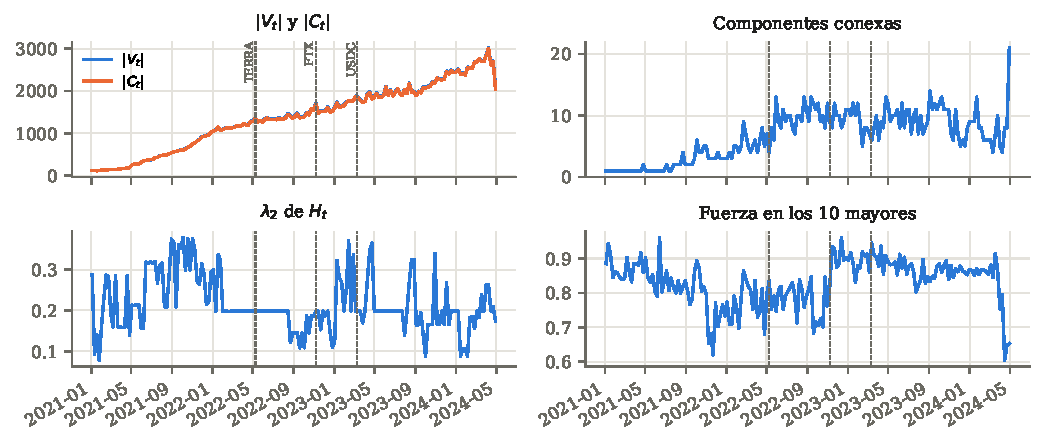
\includegraphics[width=\textwidth]{fig_caracterizacion.pdf}
\caption{La red semana a semana, de 2021 a 2024. Las líneas verticales marcan
Terra/Luna, FTX y USDC.}
\label{fig:caracterizacion}
\end{figure*}

\subsection{Qué regla causa más daño}

La Fig.~\ref{fig:curvas} y la Tabla~\ref{tab:k10} dan la respuesta. Depende de
cómo se mida el daño.

\emph{Si se cuentan protocolos desconectados}, ganan las reglas estructurales.
Con $k=10$, la articulación es la mejor en 12 de las 13 semanas y siempre supera
a la fuerza de exposición.

\emph{Si se mide la exposición que se pierde}, ganan las reglas de tamaño: la
fuerza y el CDS. Intermediación, articulación y espectral quedan por debajo de la
fuerza en todas las semanas.

Quitar protocolos al azar casi no hace daño con ninguna de las dos medidas.

\begin{figure*}[!t]
\centering
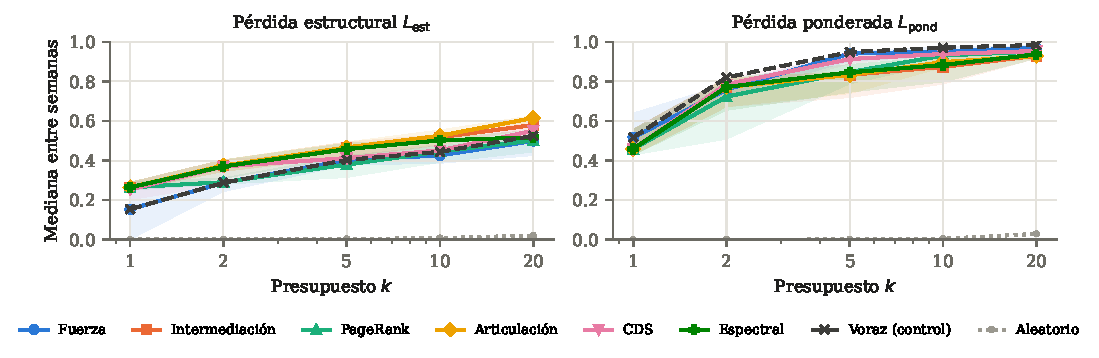
\includegraphics[width=\textwidth]{fig_curvas.pdf}
\caption{Daño según el número $k$ de protocolos quitados. La línea es la
mediana de las 13 semanas y la banda muestra la variación entre semanas.
\emph{Voraz} es un control que en cada paso quita el protocolo que más
exposición retira.}
\label{fig:curvas}
\end{figure*}

\begin{table}[!t]
\renewcommand{\arraystretch}{1.2}
\caption{Daño promedio al quitar $k=10$ protocolos y semanas en que cada regla
fue la mejor}
\label{tab:k10}
\centering
\setlength{\tabcolsep}{4pt}
\begin{tabular}{lcccc}
\toprule
& \multicolumn{2}{c}{Protocolos desconectados}
& \multicolumn{2}{c}{Exposición perdida} \\
\cmidrule(lr){2-3}\cmidrule(lr){4-5}
Regla & daño & semanas & daño & semanas \\
\midrule
Fuerza          & 0{,}41 & 0  & \textbf{0{,}95} & 6 \\
Intermediación  & 0{,}51 & 1  & 0{,}84 & 0 \\
PageRank        & 0{,}43 & 0  & 0{,}92 & 0 \\
Articulación    & \textbf{0{,}52} & 12 & 0{,}87 & 0 \\
CDS             & 0{,}45 & 0  & 0{,}94 & 7 \\
Espectral       & 0{,}48 & 0  & 0{,}86 & 0 \\
\midrule
Al azar         & 0{,}01 & -- & 0{,}01 & -- \\
\bottomrule
\end{tabular}
\end{table}

\subsection{Por qué las dos medidas no coinciden}

La Fig.~\ref{fig:descomposicion} separa la exposición perdida en dos partes: la
de los protocolos quitados y la que queda aislada del resto. La segunda es
casi cero en todos los casos (nunca pasa de 0{,}003).

Es decir, las reglas estructurales sí parten la red, pero lo que separan son
protocolos pequeños de la orilla. La exposición se pierde casi solo por quitar
a los protocolos grandes, y por eso ahí ganan las reglas de tamaño.

\begin{figure*}[!t]
\centering
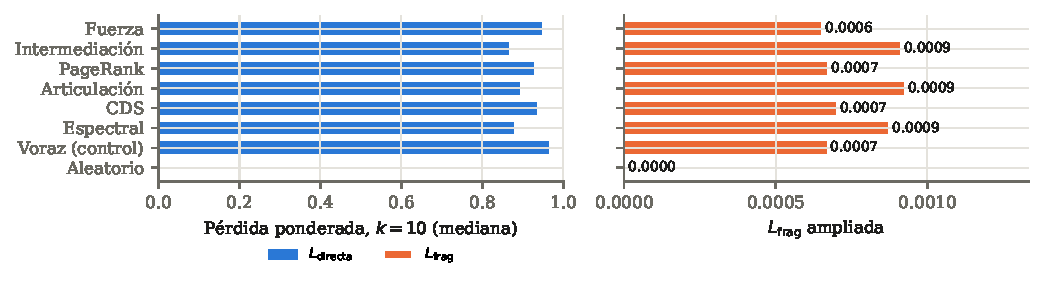
\includegraphics[width=\textwidth]{fig_descomposicion.pdf}
\caption{Exposición perdida con $k=10$, separada en la de los protocolos
quitados ($L_{\mathrm{directa}}$) y la que queda aislada
($L_{\mathrm{frag}}$). A la derecha, la segunda parte ampliada.}
\label{fig:descomposicion}
\end{figure*}

\subsection{El nodo \emph{Unknown}}
\label{sec:unknown}

Casi todas las reglas eligen primero un nodo llamado \emph{Unknown}. No es un
protocolo: es donde el panel agrupa las contrapartes que no logró identificar.
Está conectado con cerca de dos tercios de la red y concentra casi la mitad de
la exposición, o más.

Para ver si los resultados dependían de él, se repitió el estudio sin
\emph{Unknown} (sin la regla espectral, por su costo). La conclusión no cambia:
la articulación gana en protocolos desconectados las 13 semanas, y la fuerza o
el CDS ganan en exposición.

También aparecen como nodos algunas cadenas (\emph{Ethereum}, \emph{Bitcoin}) y
casas de cambio (\emph{Binance}). El panel los registra así, y los resultados
se refieren a ese panel.

\subsection{¿Eligen las reglas los mismos protocolos?}

No. La Fig.~\ref{fig:jaccard} mide cuánto se parecen los conjuntos elegidos
(1 = idénticos, 0 = sin nada en común). La fuerza y la articulación comparten
apenas una cuarta parte. Las reglas estructurales se parecen entre sí, y el CDS
se parece más a la fuerza. Hay dos familias de conjuntos, y cada una gana en su
propia medida.

\begin{figure}[!t]
\centering
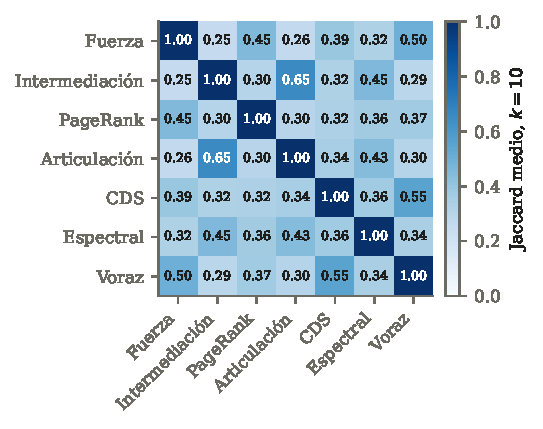
\includegraphics[width=\columnwidth]{fig_jaccard.pdf}
\caption{Parecido entre los conjuntos de 10 protocolos que elige cada regla
(índice de Jaccard, promedio de las 13 semanas).}
\label{fig:jaccard}
\end{figure}

\subsection{Comparación con TVL}

Con los datos incompletos (los faltantes contados como cero), el ranking por TVL
causa menos daño que la fuerza en las cuatro semanas disponibles. Pero los que
faltan son justamente protocolos grandes, así que este resultado no permite
sacar conclusiones.

\subsection{Los tres episodios}
\label{sec:caso}

Se marcó como afectado a todo protocolo cuya exposición cayó a la mitad o menos
en las cuatro semanas siguientes al evento. Con ese criterio, entre el 47 y el
67\,\% de la red quedó marcada, probablemente porque en esas semanas cayeron los
precios de casi todo. Ninguna regla acierta más que esa proporción de forma
constante en los tres episodios. Para decir algo útil hace falta una lista de
afectados basada en reportes públicos, que no se alcanzó a armar.

\subsection{Tiempo de cálculo}

La Fig.~\ref{fig:tiempos} muestra cuánto tarda cada regla. La fuerza y PageRank
tardan milésimas de segundo; la articulación, el CDS y la intermediación,
segundos; la espectral, hasta una hora. Todas sirven para revisar la red una vez
por semana.

\begin{figure}[!t]
\centering
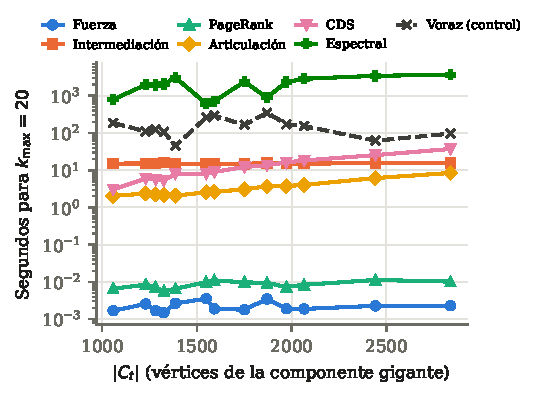
\includegraphics[width=\columnwidth]{fig_tiempos.pdf}
\caption{Segundos que tarda cada regla en elegir 20 protocolos, según el tamaño
de la red (escala logarítmica).}
\label{fig:tiempos}
\end{figure}

\section{Conclusiones}

La pregunta era si los criterios estructurales encuentran mejor que los de
tamaño a los protocolos críticos. La respuesta depende de qué se quiera evitar.

Si lo que importa es que la red no se parta, las reglas estructurales son
mejores, sobre todo la articulación. Si lo que importa es la exposición en
juego, son mejores las de tamaño. Las reglas estructurales parten la red, pero
por la orilla, donde hay poca exposición.

El CDS queda en el medio: busca entre pocos candidatos y aun así compite con la
fuerza en exposición. Estos resultados se mantienen al quitar el nodo
\emph{Unknown}.

Queda pendiente armar la lista de afectados en los tres episodios, conseguir el
TVL completo y medir el daño con contagio entre protocolos (por ejemplo, con
DebtRank \cite{battiston2012debtrank}). La herramienta \texttt{critset}
acompaña este documento y reproduce todas las cifras.


% \section*{Agradecimientos}

% Se agradece al profesor Pedro Mario Wightman Rojas, cuyo trabajo doctoral en
% control de topología \cite{wightman2010topology} proporciona el aparato
% algorítmico que este proyecto traslada a un grafo de naturaleza distinta.
\bibliographystyle{IEEEtran}
\bibliography{referencias}

\end{document}
